% Created 2019-09-26 Thu 16:26
% Intended LaTeX compiler: pdflatex
\documentclass[11pt]{article}
\usepackage[utf8]{inputenc}
\usepackage[T1]{fontenc}
\usepackage{graphicx}
\usepackage{grffile}
\usepackage{longtable}
\usepackage{wrapfig}
\usepackage{rotating}
\usepackage[normalem]{ulem}
\usepackage{amsmath}
\usepackage{textcomp}
\usepackage{amssymb}
\usepackage{capt-of}
\usepackage{hyperref}
\usepackage{amsmath}
\usepackage{esint}
\usepackage[english, russian]{babel}
\usepackage{mathtools}
\usepackage{amsthm}
\usepackage{tabu}
\usepackage[top=0.8in, bottom=0.75in, left=0.625in, right=0.625in]{geometry}
\author{Sergey Makarov}
\date{\today}
\title{}
\hypersetup{
 pdfauthor={Sergey Makarov},
 pdftitle={},
 pdfkeywords={},
 pdfsubject={},
 pdfcreator={Emacs 26.3 (Org mode 9.1.9)}, 
 pdflang={English}}
\begin{document}

Собственные значения и собственные функции ЗШЛ с разными краевыми условиями:
\begin{equation*}
\begin{tabu}{ |c|c|c| }
type    & \lambda_n & X_n \\
I - I   & \left(\frac{\pi n}{l}\right)^2 & \sin\frac{\pi n}lx \\
I - II  & \left(\frac{\pi(2n + 1)}{2l}\right)^2 & \sin\frac{\pi(2n + 1)}{2l} \\
II - I  & \left(\frac{\pi(2n + 1)}{2l}\right)^2 & \cos\frac{\pi(2n + 1)}{2l} \\
II - II & \left(\frac{\pi n}l\right)^2 & \cos\frac{\pi n}lx.
\end{tabu}
\end{equation*}

\section{Задача 3.7}
\label{sec:orga72c74c}
Решить задачу
\begin{equation}
\begin{dcases}
u_t = a^2u_{xx}, 0 < x < l, t > 0, \\
u(0, t) = 0, u(l, t) = 0, t > 0, \\
u(x, 0) = \sin\frac{\pi}lx, 0 \leq x \leq l.
\end{dcases}
\end{equation}
Найти $\lim_{t \to +\infty}u(x, t)$.

\subsection{Решение}
\label{sec:orgf9abb2b}
Собственные значения и собственные функции соответствующей задачи Штурма-Лиувилля:
\begin{equation}
\begin{cases}
\lambda_n = \left(\frac{\pi n}l\right)^2, \\
X_n = \sin\frac{\pi n}lx.
\end{cases}
\end{equation}

Общее решение ищем в виде:
\begin{equation*}
u(x, t) = \sum_{n = 0}^{\infty}C_ne^{-\lambda_na^2t}\sin\frac{\pi n}lx.
\end{equation*}
Подставим в начальное условие:
\begin{equation*}
u(x, 0) = \sum_{n = 0}^{\infty}C_n\sin\frac{\pi n}lx = \sin\frac{\pi}lx,
\end{equation*}
откуда $C_1 = 1, C_n = 0 , n \neq 1$ и окончательно:
\begin{equation}
u(x, t) = \exp\left\{-\left(\frac{\pi a}l\right)^2t\right\}\sin\frac{\pi}lx
\end{equation}
Тогда $\lim_{t \to +\infty}u(x, t) = 0$.
\section{Задача 3.9}
\label{sec:org5950be0}
Решить задачу
\begin{equation}
\begin{cases}
u_t = a^2u_{xx}, 0 < x < \pi, t > 0, \\
u(0, t) = 0, u_x(\pi, t) = 0, t > 0, \\
u(x, 0) = \sin\frac{5x}2, 0 \leq x \leq \pi.
\end{cases}
\end{equation}
Найти $\lim_{t \to +\infty}u(x, t)$. Нарисовать график $u(\pi, t)$.
\subsection{Решение}
\label{sec:orgaac21f5}
Собственные значения и собственные функции задачи Штурма-Лиувилля:
\begin{equation*}
\begin{cases}
\lambda_n = \left(\frac{2n + 1}2\right)^2, \\
X_n = \sin\frac{2n + 1}2x.
\end{cases}
\end{equation*}

Общее решение будем искать в виде:
\begin{equation*}
u(x, t) = \sum_{n = 0}^{\infty}C_ne^{-\lambda_na^2t}\sin\frac{2n + 1}2x.
\end{equation*}
Подставив в начальное условие, получим:
\begin{equation*}
u(x, 0) = \sum_{n = 0}^{\infty}C_n\sin\frac{2n + 1}2x = \sin\frac{5x}2.
\end{equation*}
Откуда $C_2 = 1, C_n = 0, n \neq 2$. Итого получаем:
\begin{equation}
u(x, t) = \exp\left\{-\left(\frac{5a}2\right)^2t\right\}\sin\frac{5x}2.
\end{equation}
Откуда $\lim_{t \to +\infty}u(x, t) = 0, u(\pi, t) = \exp\left\{-\left(\frac{5\pi}2\right)^2t\right\}\sin\frac{5\pi}2$:
\begin{figure}[htbp]
\centering
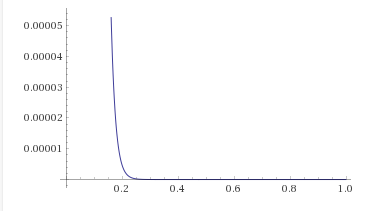
\includegraphics[width=.9\linewidth]{./img/image_2019-09-21_19-20-42.png}
\caption{график функции \(u(\pi, t)\)}
\end{figure}
\section{Задача 3.10}
\label{sec:org4f4a6e0}
Решить задачу
\begin{equation}
\begin{cases}
u_t = a^2u_{xx}, 0 < x < 1, t > 0, \\
u_x(0, t) = 0, u_x(1, t) = 0, t > 0, \\
u(x, 0) = x, 0 \leq x \leq 1.
\end{cases}
\end{equation}
Найти $\lim_{t \to +\infty}u(x, t)$.
\subsection{Решение}
\label{sec:orgdaa3dc3}
Собственные значения и собственные функции задачи Штурма-Лиувилля:
\begin{equation*}
\begin{cases}
\lambda_n = \left(\pi n\right)^2, \\
X_n = \cos\pi nx.
\end{cases}
\end{equation*}

Тогда общее решение ищем в виде
\begin{equation*}
u(x, t) = \sum_{n = 0}^{\infty}C_ne^{-\lambda_na^2t}\cos\pi nx
\end{equation*}
Подставляя в начальное условие, получим:
\begin{equation*}
u(x, 0) = \sum_{n = 0}^{\infty}C_n\cos\pi nx = x
\end{equation*}
Найдём коэффициенты $C_n$:
\begin{equation*}
C_0 = 2\int_0^1xdx = 1,
\end{equation*}
\begin{multline*}
C_n = 2\int_0^1x\cos\pi nxdx = \frac2{\pi n}\int_0^1xd(\sin\pi nx) = \frac2{\pi n}(x\sin\pi nx|_0^1 - \int_0^1\sin\pi nxdx) = \\
= \frac2{(\pi n)^2}\cos\pi nx|_0^1 = \frac2{(\pi n)^2}((-1)^n - 1) =
\begin{cases}
0, n = 2k, k \in \mathbb{Z}, \\
\left(\frac2{\pi n}\right)^2, n = 2k + 1, k \in \mathbb{Z}.
\end{cases}
\end{multline*}
Итого получаем
\begin{equation}
u(x, t) = 1 + \sum_{n = 0}^{\infty}\left(\frac2{\pi(2n + 1)}\right)^2e^{-(\pi(2n + 1)a)^2t}\cos\pi(2n + 1)x.
\end{equation}
Откуда $\lim_{t \to +\infty}u(x, t) = 1$.
\section{Задача 3.11}
\label{sec:orgaec3cee}
Решить задачу
\begin{equation}
\begin{cases}
u_t = a^2u_{xx}, 0 < x < 1, t > 0, \\
u(0, t) = u_1, u(1, t) = u_2, \\
u(x, 0) = u_0x, 0 \leq x \leq 1.
\end{cases}
\end{equation}
Найти $\lim_{t \to +\infty}u(x,t)$.
\subsection{Решение}
\label{sec:org3f94063}
Найдём решение в виде \(u(x, t) = U(x, t) + v(x, t)\), где \(U(x, t) = a(t)x + b(t)\).
Подставляя в граничные условия, получим:
   \begin{equation*}
   \begin{cases}
   b(t) = u_1, \\
   a(t) + b(t) = u_2
   \end{cases}
   \Rightarrow
   \begin{cases}
   a(t) = u_2 - u_1, \\
   b(t) = u_1.
   \end{cases}
   \end{equation*}
   Откуда $u(x, t) = v(x, t) + (u_0 - u_1)x + u_1$. Подставляя это выражение в (7), получим:
\begin{equation}
\begin{cases}
v_t = a^2v_{xx}, 0 < x < 1, t > 0, \\
v(0, t) = v(1, t) = 0, \\
v(x, 0) = u_0x - (u_2 - u_1)x - u_1 = (u_0 + u_1 - u_2)x - u_1.
\end{cases}
\end{equation}
Собственные значения и собственные функции для соответствующей задачи Штурма-Лиувилля будут:
\begin{equation*}
\begin{cases}
\lambda_n = \left(\pi n\right)^2, \\
X_n = \sin\pi nx.
\end{cases}
\end{equation*}
Ищем решение задачи (8) в виде
\begin{equation*}
v(x, t) = \sum_{n = 0}^{\infty}C_ne^{-\lambda_na^2t}\sin\pi nx.
\end{equation*}
Подставляя это представление в начальное условие, получим:
\begin{equation*}
v(x, 0) = \sum_{n = 0}^{\infty}C_n\sin\pi nx = (u_0 + u_1 - u_2)x - u_1.
\end{equation*}
Заметим, что подставив в (7) или (8) точку $(0, 0)$, можно получить, что $u_1 = 0$.
Исходя из этого, получим коэффициенты $C_n$:
\begin{multline*}
C_n = \int_0^1(u_0 - u_2)x\sin\pi nxdx = -\frac{u_0 - u_2}{\pi n}\int_0^1x(d\cos\pi nx) =
\frac{u_2 - u_0}{\pi n}(x\cos\pi nx|_0^1 - \int_0^1\cos\pi nxdx) = \\
= \frac{u_2 - u_0}{\pi n}\left((-1)^n - \frac1{\pi n}\sin\pi nx|_0^1\right) =
(-1)^n\frac{u_2 - u_0}{\pi n}
\end{multline*}
Итого для $u(x, t)$ получаем:
\begin{equation}
u(x, t) = u_0x + \frac{u_2 - u_0}{\pi n}\sum_{n = 0}^{\infty}(-1)^ne^{-(\pi na)^2t}\sin{\pi nx}
\end{equation}
В данном случае $\lim_{t \to +\infty}u(x, t) = u_0x$.
\section{Задача 3.12}
\label{sec:orga655241}
Решить задачу
\begin{equation}
\begin{cases}
u_t = a^2u_{xx} - b(u - U), 0 < x < l, t > 0, b > 0, \\
u_x(0, t) = 0, u(l, t) = U, t > 0, \\
u(x, 0) = u_0, 0 \leq x \leq l.
\end{cases}
\end{equation}
Найти $\lim_{t \to +\infty}u(x, t)$.
\subsection{Решение}
\label{sec:org5fe4c18}
Для начала приведём задачу к однородной. Для этого будем искать решение задачи (10) в виде
\(u(x, t) = U(x, t) + v(x, t)\), где \(U(x, t) = a(t)x + b(t)\). Подставляя это представление в
граничные условия, найдём:
\begin{equation*}
\begin{cases}
a(t) = 0, \\
a(t)l + b(t) = U
\end{cases}
\Rightarrow
\begin{cases}
a(t) = 0, \\
b(t) = U.
\end{cases}
\end{equation*}
Таким образом, $u(x, t) = v(x, t) + U$. Подставив это представление в (10), получим однородную
задачу для $v(x, t)$:
\begin{equation}
\begin{cases}
v_t = a^2v_{xx} - bv, 0 < x < l, t > 0, b > 0, \\
v_x(0, t) = v(l, t) = 0, \\
v(x, 0) = u_0 - U, 0 \leq x \leq l.
\end{cases}
\end{equation}
Решение этой задачи будем искать в виде $v(x, t) = X(x)T(t)$. Подставив это представление в (11),
получим:
\begin{equation*}
X(x)T'(t) = a^2X''(x)T(t) - bX(x)T(t) \Rightarrow X(x)(T'(t) + bT(t)) = a^2X''(x)T(t) \Rightarrow
\frac{X''}{X} = \frac{T'(t) + bT(t)}{a^2T(t)} = -\lambda.
\end{equation*}
Получили задачу Штурма-Лиувилля для $X(x)$:
\begin{equation}
\begin{cases}
X'' + \lambda X = 0, \\
X'(0) = X(l) = 0.
\end{cases}
\end{equation}
и уравнение для $T(t)$:
\begin{equation}
T'(t) + (b + \lambda a^2)T(t) = 0.
\end{equation}
Собственные значения и собственные функции задачи (12) имеют вид:
\begin{equation*}
\begin{dcases}
\lambda_n = \left(\frac{\pi(2n + 1)}{2l}\right)^2, \\
X_n = \cos\frac{\pi(2n + 1)}{2l}x.
\end{dcases}
\end{equation*}
Решение уравнения (13) имеет вид:
\begin{equation*}
T(t) = Ce^{-(b + \lambda_na^2)t}
\end{equation*}
Поэтому общее решение задачи (11) ищем в виде ряда:
\begin{equation}
v(x, t) = \sum_{n = 0}^{\infty}C_ne^{-(b + \lambda_na^2)t}\cos\frac{\pi(2n + 1)}{2l}x.
\end{equation}
Подставив (14) в начальное условие, получим:
\begin{equation*}
v(x, 0) = \sum_{n = 0}^{\infty}C_n\cos\frac{\pi(2n + 1)}{2l}x = u_0 - U.
\end{equation*}
Найдём коэффициенты $C_n$:
\begin{multline*}
C_n = \frac2l\int_0^l(u_0 - U)\cos\frac{\pi(2n + 1)}{2l}xdx =
\frac2l\frac{2l}{\pi(2n + 1)}(u_0 - U)\sin\frac{\pi(2n + 1)}{2l}x\bigg|_0^l =
\frac{4(u_0 - U)}{\pi(2n + 1)}\sin\frac{\pi(2n + 1)}2
\end{multline*}
Откуда находим окончательный вид для $u(x, t)$:
\begin{equation}
u(x, t) = U + \sum_{n = 0}^{\infty}\frac{4(u_0 - U)}{\pi(2n + 1)}\sin\frac{\pi(2n + 1)}2
\exp\left\{-\left(b + \left(\frac{\pi(2n + 1)a}{2l}\right)^2\right)t\right\}\cos\frac{\pi(2n + 1)}{2l}x.
\end{equation}
Отсюда $\lim_{t \to +\infty}u(x, t) = U$.
\end{document}
